\chapter*{Appendix}
\label{chap:appendix}

\vspace*{-16pt}
\refstepcounter{section}
\section*{\thesection \quad Links to Workflows and Additional Materials}
\hspace*{-18pt}All workflows in Galaxy-specific GA and CWL formats are available on GitHub:\\
\url{https://github.com/kciy/msc-thesis/tree/main/workflows/}

\refstepcounter{subsection}
\subsection*{\thesubsection \quad Poxvirus Workflow}
\label{sec:apx-pox-links}

\begin{itemize}
	\setlength{\itemsep}{-0.4cm}
	\item Galaxy EU:\\
	\url{https://usegalaxy.eu/u/vyetoria/w/pox-virus-illumina-amplicon}
	\item GitHub Intergalactic Workflow Commission:\\
	\url{https://github.com/galaxyproject/iwc/tree/main/workflows/virology/pox-virus-amplicon}
	\item WorkflowHub:\\
	\url{https://workflowhub.eu/workflows/439}
	\item Dockstore:\\
	\url{https://dockstore.org/workflows/github.com/iwc-workflows/pox-virus-amplicon/main:main?tab=info}
	\item Galaxy Training Material:\\
	\url{https://training.galaxyproject.org/training-material/topics/variant-analysis/tutorials/pox-tiled-amplicon/tutorial.html}
	\item Galaxy history with workflow test run (\ac{LSDV} samples 20L70 and 20L81):\\
	\url{https://usegalaxy.eu/u/vyetoria/h/pox-virus-illumina-amplicon-sample-lsdv} 
\end{itemize}

\refstepcounter{subsection}
\subsection*{\thesubsection \quad Avian Influenza Virus Workflow}
\label{sec:apx-aiv-links}

\begin{itemize}
	\setlength{\itemsep}{-0.4cm}
	\item Galaxy EU:\\
	\url{https://usegalaxy.eu/u/vyetoria/w/aiv-illumina-analysis}
	\item Reference Database:\\
	\url{https://usegalaxy.eu/u/vyetoria/h/aiv-reference-sequences}
	\item Galaxy Training Material:\\
	\url{https://training.galaxyproject.org/training-material/topics/variant-analysis/tutorials/aiv-analysis/tutorial.html}
	\item Galaxy history with workflow test run (H4N6 sample):\\
	\url{https://usegalaxy.eu/u/vyetoria/h/aiv-seq-analysis-test-h4n6}
	\item Galaxy history with workflow test run (H5N8 sample):\\
	\url{https://usegalaxy.eu/u/vyetoria/h/aiv-seq-analysis-test-h5n8}
\end{itemize}

\refstepcounter{subsection}
\subsection*{\thesubsection \quad Foot-and-mouth Disease Virus Workflows}
\label{sec:apx-fmdv-links}

\begin{itemize}
	\setlength{\itemsep}{-0.4cm}
	\item Part 1 (\textit{De novo} assembly and BLASTn search) Galaxy EU:\\
	\url{https://usegalaxy.eu/u/vyetoria/w/fmdv-sequence-analysis-part-1-assembly-and-blastn-search}
	\item Part 2 (Mapping and consensus sequence construction) Galaxy EU:\\
	\url{https://usegalaxy.eu/u/vyetoria/w/fmdv-sequence-analysis-part-2-mapping-consensus}
	\item Galaxy history with workflow 1 test run (SRR17960053, SRR18751245, SRR18685689 and SRR9328470):\\
	\url{https://usegalaxy.eu/u/vyetoria/h/fmdv-sequence-analysis-1-2}
	\item Galaxy histories of workflow 2 test runs:
	\begin{itemize}
		\setlength{\itemsep}{-0.4cm}
		\vspace*{-0.4cm}
		\item SRR17960053 (Asia-1 sample):\\
		\url{https://usegalaxy.eu/u/vyetoria/h/fmdv-seq-analysis-2-2-asia-1}
		\item SRR18751245 (A sample):\\
		\url{https://usegalaxy.eu/u/vyetoria/h/fmdv-seq-analysis-2-2-a}
		\item SRR18685689 (SAT-1 sample):\\
		\url{https://usegalaxy.eu/u/vyetoria/h/fmdv-seq-analysis-2-2-sat-1}
		\item SRR9328470 (SAT-2 sample):\\
		\url{https://usegalaxy.eu/u/vyetoria/h/fmdv-seq-analysis-2-2-sat-2}
	\end{itemize}
\end{itemize}

\refstepcounter{subsection}
\subsection*{\thesubsection \quad Links to Tool Wrappers}
\label{sec:apx-wrap-links}

These tools have been wrapped in the Galaxy Tools IUC to make them available on the Galaxy EU server instance.

\begin{itemize}
	\setlength{\itemsep}{-0.4cm}
	\item \texttt{snipit} XML Tool Wrapper:\\
	\url{https://github.com/galaxyproject/tools-iuc/tree/main/tools/snipit}
	\item \texttt{VAPOR} XML Tool Wrapper:\\
	\url{https://github.com/galaxyproject/tools-iuc/tree/main/tools/vapor}
	\item \texttt{UCSC faToVcf} XML Tool Wrapper:\\
	\url{https://github.com/galaxyproject/tools-iuc/tree/main/tools/ucsc_tools/fatovcf}
\end{itemize}

\newpage
\refstepcounter{section}
\section*{\thesection \quad Reference Collection for AIV Workflow}
\refstepcounter{subsection}
\subsection*{\thesubsection \quad Filter Criteria and Amount of Sequences}
\setlength{\tabcolsep}{8pt}
\renewcommand{\arraystretch}{1.3}
\begin{table}[ht!]
	\centering
	\begin{tabular}{@{}llcccccc@{}}
	\hline
					 &                   & \multicolumn{1}{l|}{}                                                           & \multicolumn{2}{c|}{\textbf{Filter criteria \textsuperscript{1}}}                                                                                                                    & \multicolumn{3}{c}{\textbf{Reference collection}}                                                                                                                                                \\ \hline
	\multicolumn{2}{l}{Segment} & \multicolumn{1}{l|}{Length \textsuperscript{2}} & \multicolumn{1}{l}{\begin{tabular}[c]{@{}l@{}}Minimum\\ length\end{tabular}} & \multicolumn{1}{l|}{\begin{tabular}[c]{@{}l@{}}Maximum\\ length\end{tabular}} & \multicolumn{1}{l}{\begin{tabular}[c]{@{}l@{}}\# of\\ sequences\end{tabular}} & \multicolumn{1}{l}{Length range} & \multicolumn{1}{l}{\begin{tabular}[c]{@{}l@{}}Mean\\ length\end{tabular}} \\ \hline
	1                & PB2               & \multicolumn{1}{c|}{2 316}                                                      & 1 945                                                                          & \multicolumn{1}{c|}{2 432}                                                      & 17 714                                                                        & 2 244 - 2 417                      & 2 306.7                                                                     \\
	2                & PB1               & \multicolumn{1}{c|}{2 316}                                                      & 1 945                                                                          & \multicolumn{1}{c|}{2 432}                                                      & 17 355                                                                        & 2 265 - 2 414                      & 2 304.9                                                                     \\
	3                & PA                & \multicolumn{1}{c|}{2 208}                                                      & 1 766                                                                          & \multicolumn{1}{c|}{2 318}                                                      & 17 569                                                                        & 1 905 - 2 275                      & 2 192.4                                                                     \\
	\textbf{4}       & \textbf{HA}       & \multicolumn{1}{c|}{\textbf{1 752}}                                             & \textbf{1 401}                                                                 & \multicolumn{1}{c|}{\textbf{1 840}}                                             & \textbf{20 753}                                                               & \textbf{1 659 - 1 805}             & \textbf{1 717.5}                                                            \\
	5                & NP                & \multicolumn{1}{c|}{1 540}                                                      & 1 232                                                                          & \multicolumn{1}{c|}{1 617}                                                      & 16 024                                                                        & 1 440 - 1 616                      & 1 529.9                                                                     \\
	\textbf{6}       & \textbf{NA}       & \multicolumn{1}{c|}{\textbf{1 434}}                                             & \textbf{1 147}                                                                 & \multicolumn{1}{c|}{\textbf{1 506}}                                             & \textbf{17 646}                                                               & \textbf{1 308 - 1 498}             & \textbf{1 418.8}                                                            \\
	7                & MP                & \multicolumn{1}{c|}{1 002}                                                      & 801                                                                            & \multicolumn{1}{c|}{1 052}                                                      & 14 684                                                                        & 979 - 1 047                        & 1 001.0                                                                     \\
	8                & NS                & \multicolumn{1}{c|}{865}                                                        & 692                                                                            & \multicolumn{1}{c|}{908}                                                        & 15 762                                                                        & 752 - 907                          & 860.9                                                                       \\ \hline
	\multicolumn{8}{l}{\begin{tabular}[c]{@{}l@{}}\textsuperscript{1} Minimum cutoff length is 80\% of segment length, maximal cutoff length is \\105\% of segment length.\\\textsuperscript{2} For strain A/swine/Iowa/18Tosu0505/2018(H1N1)~\cite{chauhan2022overview}.\\\end{tabular}}                                                
	\end{tabular}
	\caption{Summary of reference collection obtained from search criteria on the NCBI Influenza Virus Database.}
 \label{tab:apx-aiv-ref}
\end{table}
\newpage
\refstepcounter{subsection}
\subsection*{\thesubsection \quad Reference Collection by Amount of Sequence per Subtype}
\setlength{\tabcolsep}{10pt}
\renewcommand{\arraystretch}{1.3}
\begin{table}[ht!]
	\centering
	\begin{tabular}{@{}lcclcc@{}}
	\hline
	\textbf{\begin{tabular}[c]{@{}l@{}}HA\\Subtype\end{tabular}}  & \textbf{\begin{tabular}[c]{@{}l@{}}\# of HA\\ sequences\end{tabular}}  & \textbf{\begin{tabular}[c]{@{}l@{}}\# of NA\\ sequences\end{tabular}}  & \textbf{\begin{tabular}[c]{@{}l@{}}NA\\Subtype\end{tabular}}  & \textbf{\begin{tabular}[c]{@{}l@{}}\# of HA\\ sequences\end{tabular}}  & \textbf{\begin{tabular}[c]{@{}l@{}}\# of NA\\ sequences\end{tabular}}  \\ \hline
	\textbf{H1}  & 779          & 787          & \textbf{N1}  & 4 317        & 3 797        \\
	\textbf{H2}  & 512          & 450          & \textbf{N2}  & 6 346        & 5 419        \\
	\textbf{H3}  & 1 857        & 1 724        & \textbf{N3}  & 1 585        & 1 387        \\
	\textbf{H4}  & 1 561        & 1 520        & \textbf{N4}  & 344          & 304          \\
	\textbf{H5}  & 5 199        & 4 345        & \textbf{N5}  & 523          & 442          \\
	\textbf{H6}  & 1 817        & 1 808        & \textbf{N6}  & 2 454        & 2 360        \\
	\textbf{H7}  & 1 898        & 1 655        & \textbf{N7}  & 838          & 761          \\
	\textbf{H8}  & 169          & 155          & \textbf{N8}  & 2 255        & 2 077        \\
	\textbf{H9}  & 3 530        & 2 835        & \textbf{N9}  & 1 260        & 1 092        \\
	\textbf{H10} & 866          & 851          & \textbf{N10} & 0            & 0            \\
	\textbf{H11} & 749          & 672          & \textbf{N11} & 0            & 0            \\
	\textbf{H13} & 370          & 310          &              &              &              \\
	\textbf{H14} & 42           & 38           &              &              &              \\
	\textbf{H15} & 15           & 12           &              &              &              \\
	\textbf{H16} & 225          & 177          &              &              &              \\
	\textbf{H12} & 337          & 266          &              &              &              \\
	\textbf{H17} & 0            & 0            &              &              &              \\
	\textbf{H18} & 0            & 0            &              &              &              \\ \hline
	\end{tabular}
	\caption[AIV reference collection by HA and NA subtypes.]{Amount of sequences per HA and NA gene dataset of reference sequences, divided by 18 HA and 11 NA subtypes present in the AIV reference database, retrieved from NCBI Influenza Virus Database. Subtypes H17, H18, N10 and N11 are excluded for irrelevance in livestock (H17N10 and H18N11 is only known in bats~\cite{tong2013new}).}
\label{tab:apx-aiv-ref-subtypes}
\end{table}

\begin{figure}
	\refstepcounter{section}
	\section*{\thesection \quad Results of H4N6 and H5N8 Samples for AIV Workflow}
	\centering
	\begin{subfigure}[b]{1.1\textwidth}
		\hspace*{-50pt}
		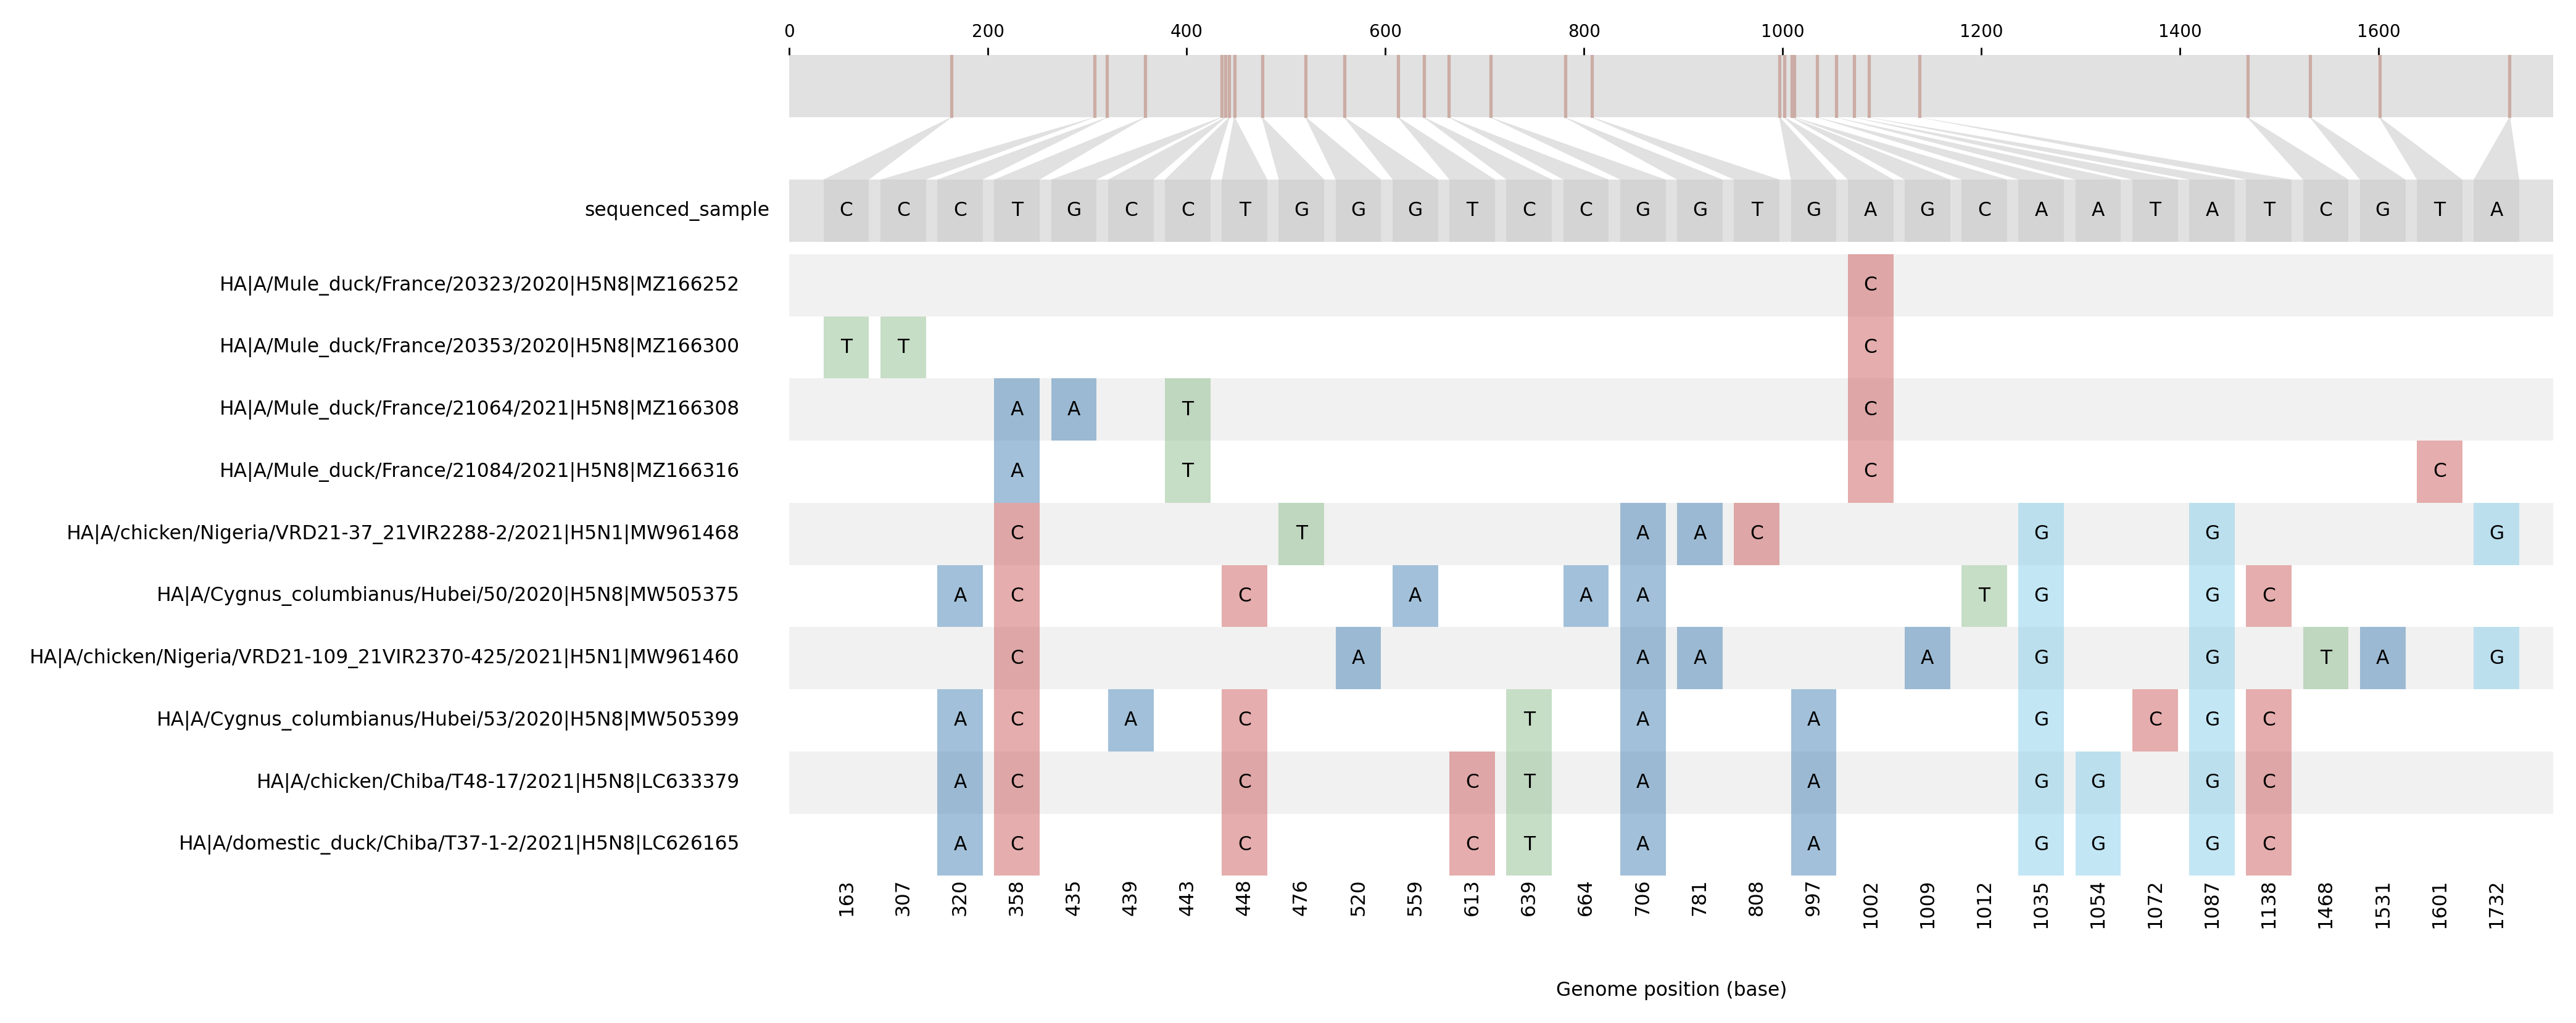
\includegraphics[width=1.0\textwidth]{media/4-aiv-snipit-s8-4-ha.png}
		\caption{SNPs of HA gene of H5N8 sample.}
		\label{fig:apx-aiv-snipit-s8-ha}
	\end{subfigure}
	\\
	\vspace*{20pt}
	\begin{subfigure}[b]{1.0\textwidth}
		\hspace*{-40pt}
		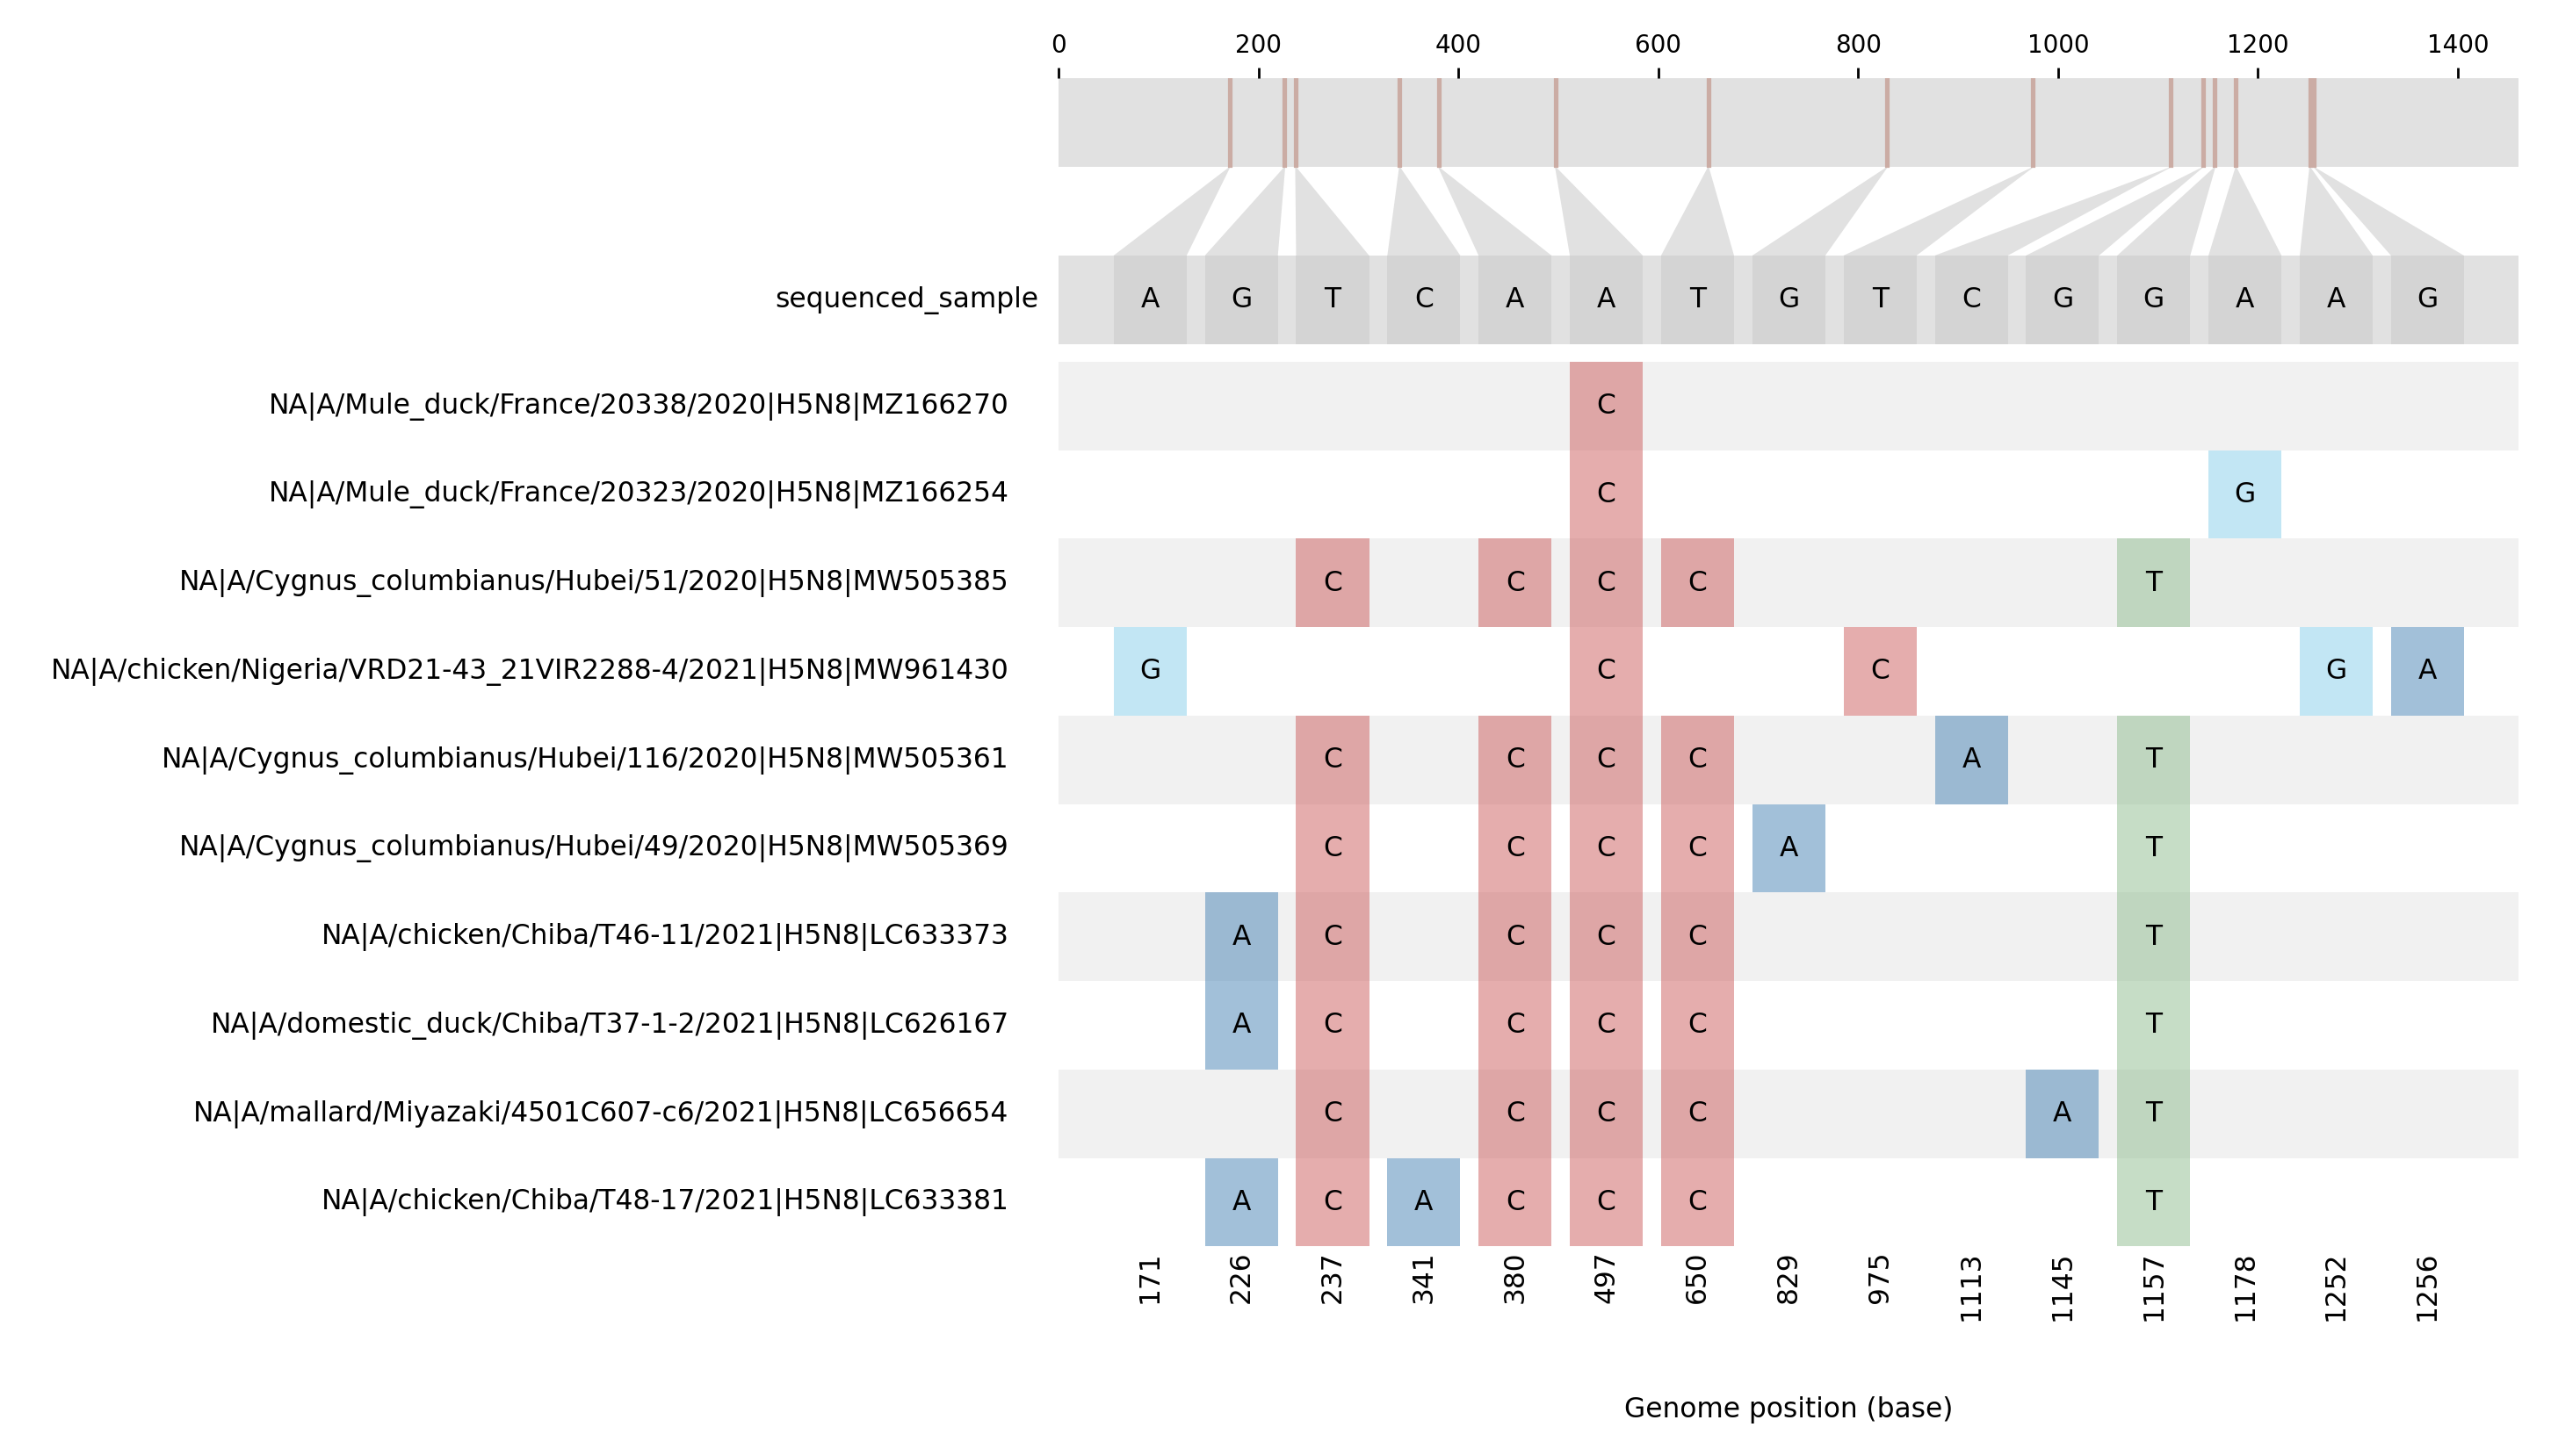
\includegraphics[width=1.0\textwidth]{media/4-aiv-snipit-s8-6-na.png}
	\caption{SNPs of NA gene of H5N8 sample.}
	\label{fig:apx-aiv-snipit-s8-na}
	\end{subfigure}
	\caption[Visual summaries of SNPs in H5N8 sample.]{Visual summaries of SNPs in H5N8 sample. The consensus sequence of the gene is the reference at the top of each plot.}
\label{fig:apx-aiv-snipit-s8}
\end{figure}

\begin{sidewaysfigure}
    \centering
    \subfloat[SNPs of HA gene of H4N6 sample.]{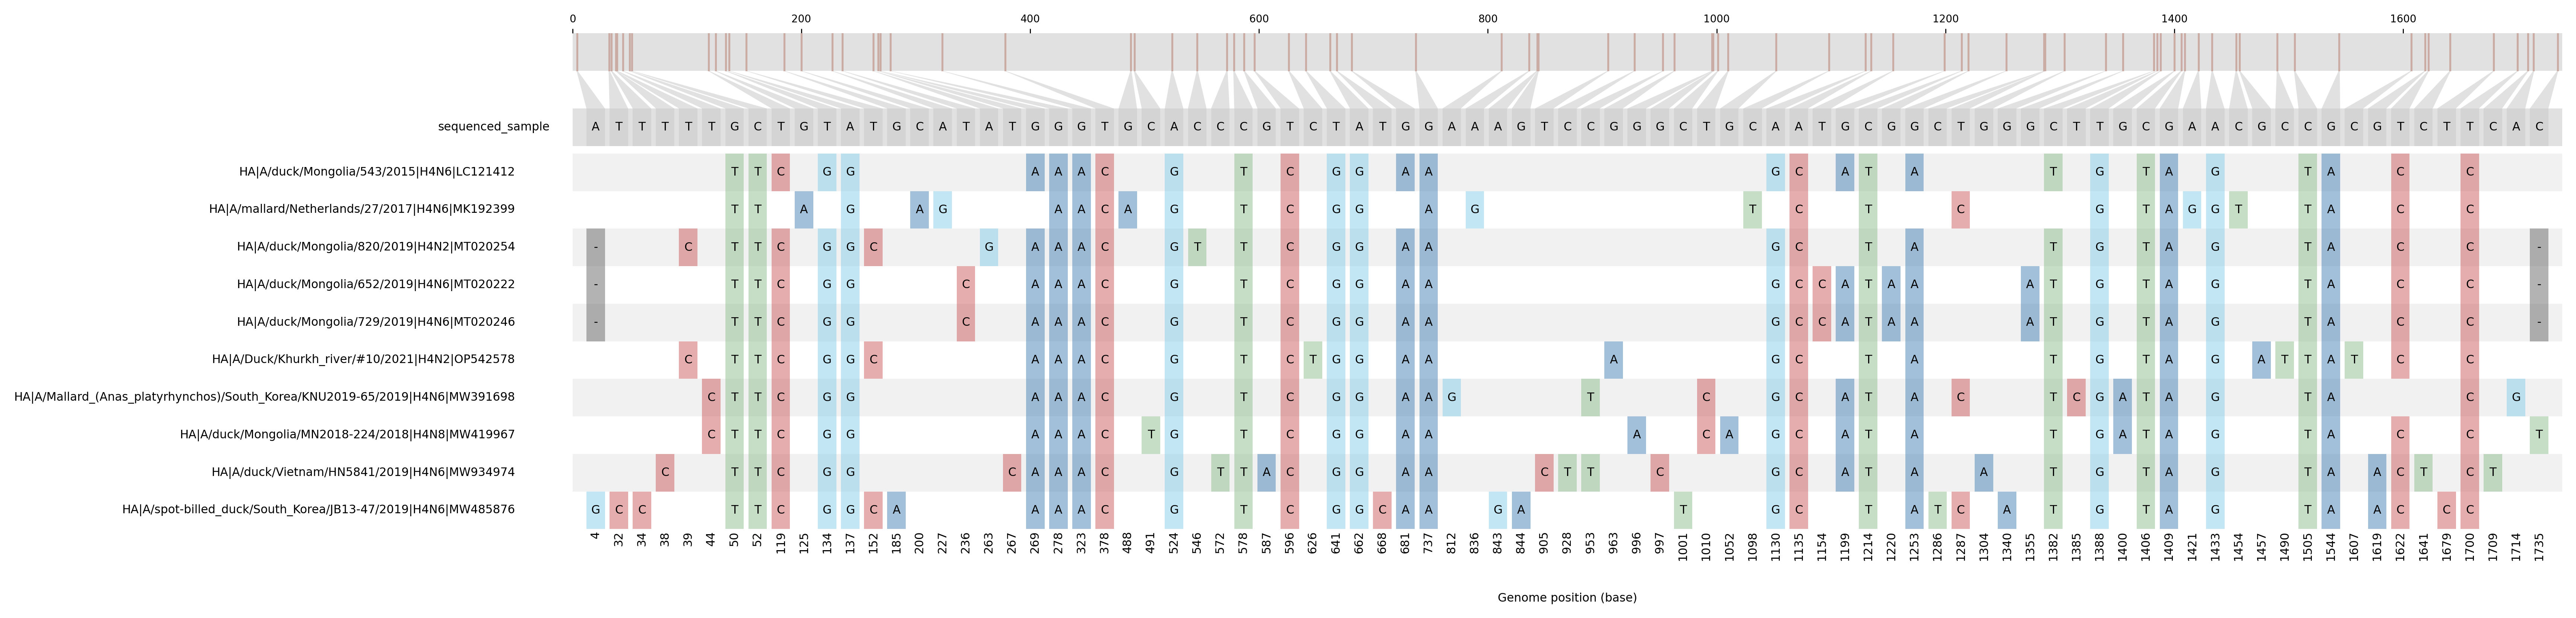
\includegraphics[width=1.0\textheight]{media/4-aiv-snipit-s4-4-ha.png}\label{fig:apx-aiv-snipit-s4-ha}} \\
    \subfloat[SNPs of NA gene of H4N6 sample.]{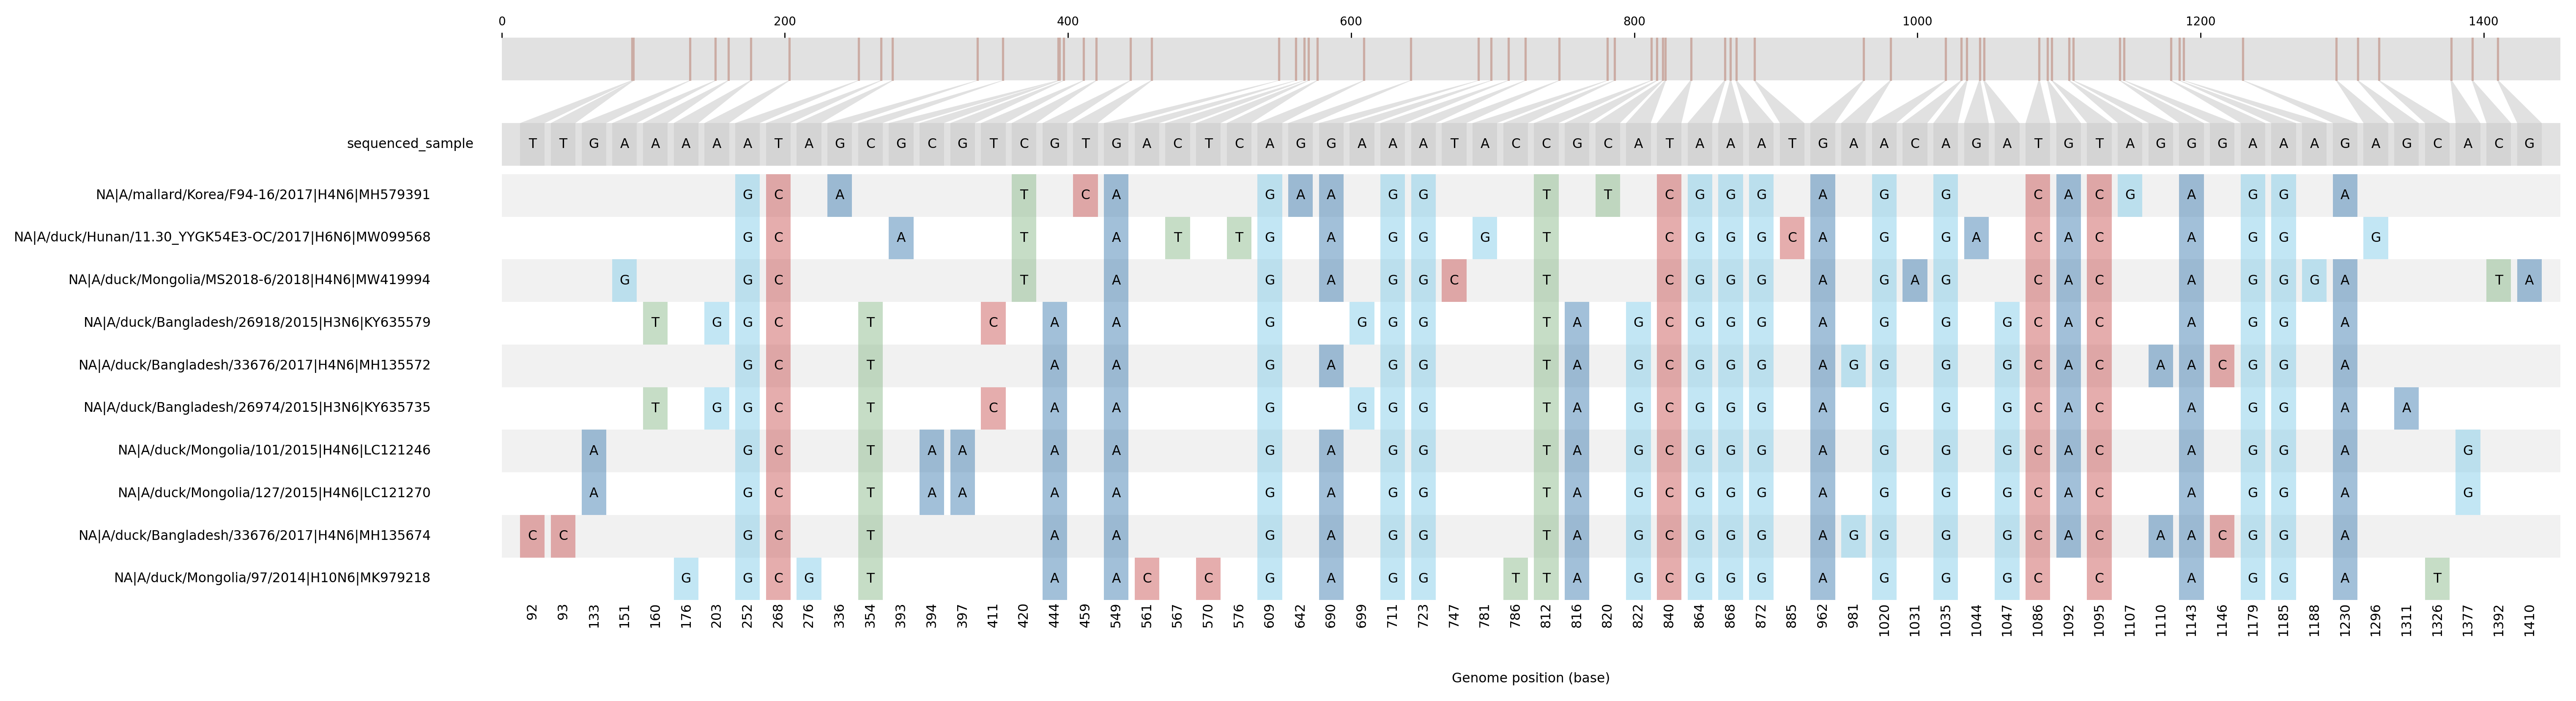
\includegraphics[width=1.0\textheight]{media/4-aiv-snipit-s4-6-na.png}\label{fig:apx-aiv-snipit-s4-na}}
    \caption[Visual summaries of SNPs in H4N6 sample.]{Visual summaries of SNPs in H4N6 sample. The consensus sequence of the gene is the reference at the top of each plot.}
\label{fig:apx-aiv-snipit-s4}
\end{sidewaysfigure}

\begin{figure}
    \centering
    \begin{subfigure}[]{0.5\textheight}
        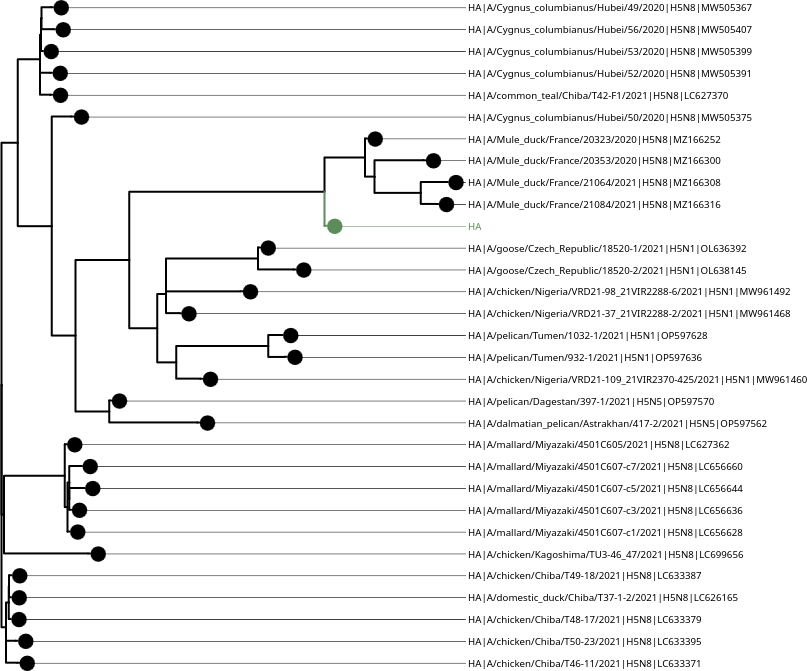
\includegraphics[width=1.0\textwidth]{media/4-aiv-s4-tree-ha.png}
        \caption{Phylogenetic tree of HA gene of H4N6 sample.}
		\label{fig:apx-aiv-trees-s4-ha}
    \end{subfigure} \\
	\vspace*{20pt}
    \begin{subfigure}[]{0.5\textheight}
        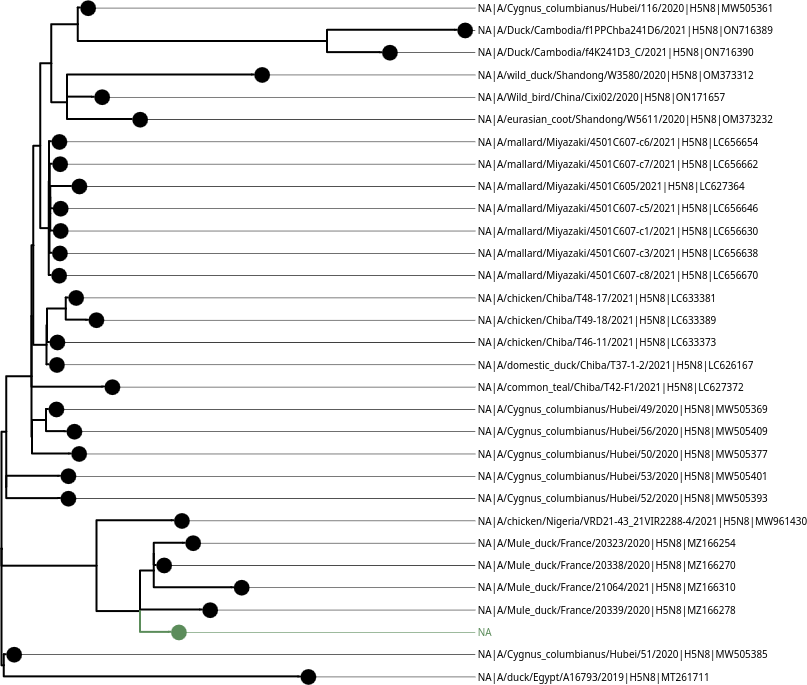
\includegraphics[width=1.0\textwidth]{media/4-aiv-s4-tree-na.png}
        \caption{Phylogenetic tree of NA gene of H4N6 sample.}
		\label{fig:apx-aiv-trees-s4-na}
    \end{subfigure} 
	\caption[Phylogenetic trees of HA and NA genes for H4N6 sample.]{Phylogenetic trees of HA and NA genes for H4N6 sample, indicating linkage to \textit{A/mallard/Netherlands} (HA) and to \textit{A/duck/Hunan} (NA). The consensus sequence is marked in green. The other sequences are the 30 highest scoring sequences from the \texttt{VAPOR} run.}
\label{fig:apx-aiv-trees-s4}
\end{figure}

\begin{figure}
    \centering
    \begin{subfigure}[]{0.5\textheight}
        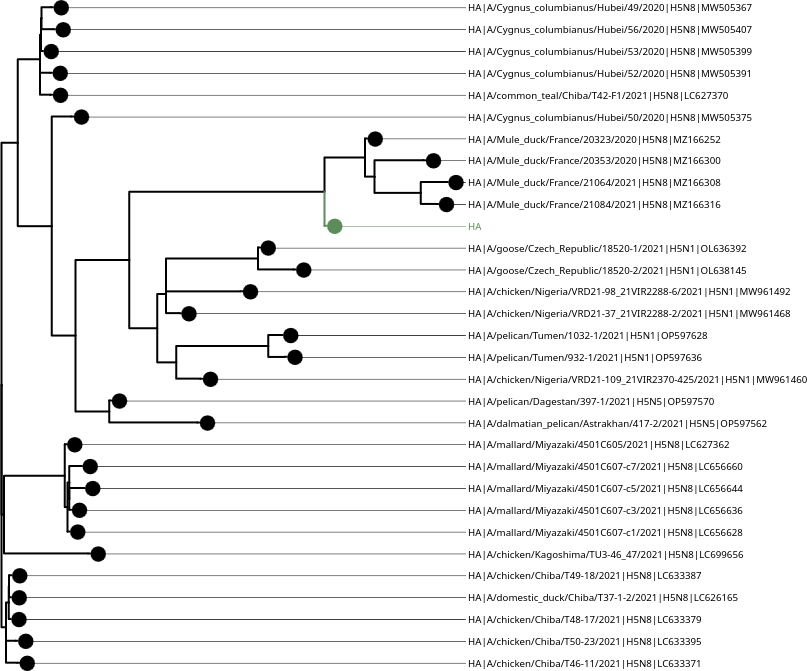
\includegraphics[width=1.0\textwidth]{media/4-aiv-s8-tree-ha.png}
        \caption{Phylogenetic tree of HA gene of H5N8 sample.}
		\label{fig:apx-aiv-trees-s8-ha}
    \end{subfigure} \\ 
	\vspace*{20pt}
    \begin{subfigure}[]{0.5\textheight}
        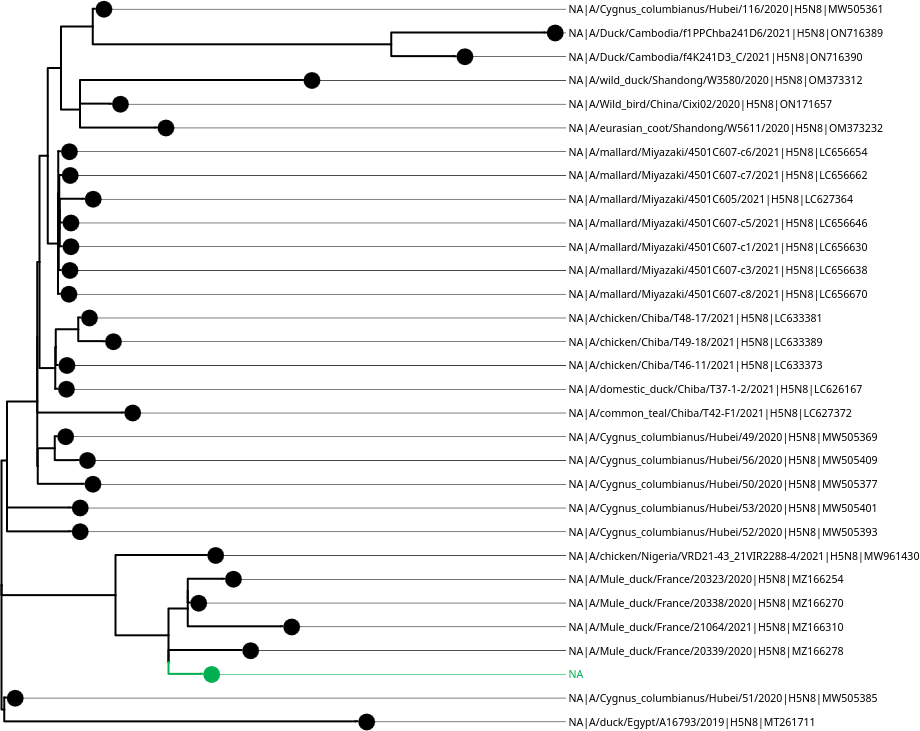
\includegraphics[width=1.0\textwidth]{media/4-aiv-s8-tree-na.png}
        \caption{Phylogenetic tree of NA gene of H5N8 sample.}
		\label{fig:apx-aiv-trees-s8-na}
    \end{subfigure} 
	\caption[Phylogenetic trees of HA and NA genes for H5N8 sample.]{Phylogenetic trees of HA and NA genes for H5N8 sample, indicating linkage to \textit{A/Mule\_duck/France} in both the HA and NA segments.}
\label{fig:apx-aiv-trees-s8}
\end{figure}

\newpage
\begin{table}[ht]
	\refstepcounter{section}
	\section*{\thesection \quad Ambiguous Sites of Consensus Sequences in LSDV Samples}
	% \centering
	\begin{tabular}{l|llc|lc}
	\hline
	\textbf{Reference}                      & \textbf{No.} & \textbf{\begin{tabular}[c]{@{}l@{}}Ambiguous sites\\ in consensus of \\ 20L81\end{tabular}} & \textbf{\begin{tabular}[c]{@{}c@{}}Length\\ {[}bases{]}\end{tabular}} & \textbf{\begin{tabular}[c]{@{}l@{}}Ambiguous sites\\ in consensus of\\ 20L70\end{tabular}} & \textbf{\begin{tabular}[c]{@{}c@{}}Length\\ {[}bases{]}\end{tabular}} \\ \hline
	\multirow{3}{*}{\textbf{\begin{tabular}[c]{@{}c@{}}LSDV-\\Herbivac\end{tabular}}} & 1            & 1--264                                                                                      & 264                                                                   & 1--264                                                                                     & 264                                                                   \\
											& 2            & 139,037--139,152                                                                            & 115                                                                   & 139,037--139,152                                                                           & 115                                                                   \\
											& 3            & 150,500--150,526                                                                            & 26                                                                    & 150,502--150,526                                                                           & 24                                                                    \\ \hline
	\multirow{5}{*}{\textbf{SPPV}}          & 4            & 1--264                                                                                      & 264                                                                   & 1--264                                                                                     & 264                                                                   \\
											& 5            & 18,479--18,498                                                                              & 19                                                                    & 18,486--18,505                                                                             & 19                                                                    \\
											& 6            & 110,083--110,106                                                                            & 23                                                                    & 110,090--110,113                                                                           & 23                                                                    \\
											& 7            &                                                                                             &                                                                       & 129,582--129,583                                                                           & 1                                                                     \\
											& 8            & 150,075--150,198                                                                            & 123                                                                   & 150,072--150,192                                                                           & 120                                                                   \\ \hline
	\multirow{3}{*}{\textbf{GTPV}}          & 9            & 1--264                                                                                      & 264                                                                   & 1--264                                                                                     & 264                                                                   \\
											& 10           & 121,520--121,521                                                                            & 1                                                                     & 121,489--121,490                                                                           & 1                                                                     \\
											& 11           & 149,959--149,973                                                                            & 14                                                                    & 149,931--149,942                                                                           & 11                                                                    \\ \hline
	\end{tabular}
	\caption[Ambiguous sites of consensus sequences in LSDV samples with varying reference.]{Ambiguous sites of consensus sequences in LSDV samples with varying reference, highlighting the equivocal positions with low coverage sites that occur due to low coverage and/or loose primer ends due to read mapping to a suboptimal reference.}
\label{tab:apx-capv-n}
\end{table}

\begin{figure}[ht!]
	\refstepcounter{section}
	\section*{\thesection \quad Results of Tool Profiling for BWA-MEM and rnaviralSPAdes Runs}
    \centering
	\begin{subfigure}[b]{1.0\textwidth}
        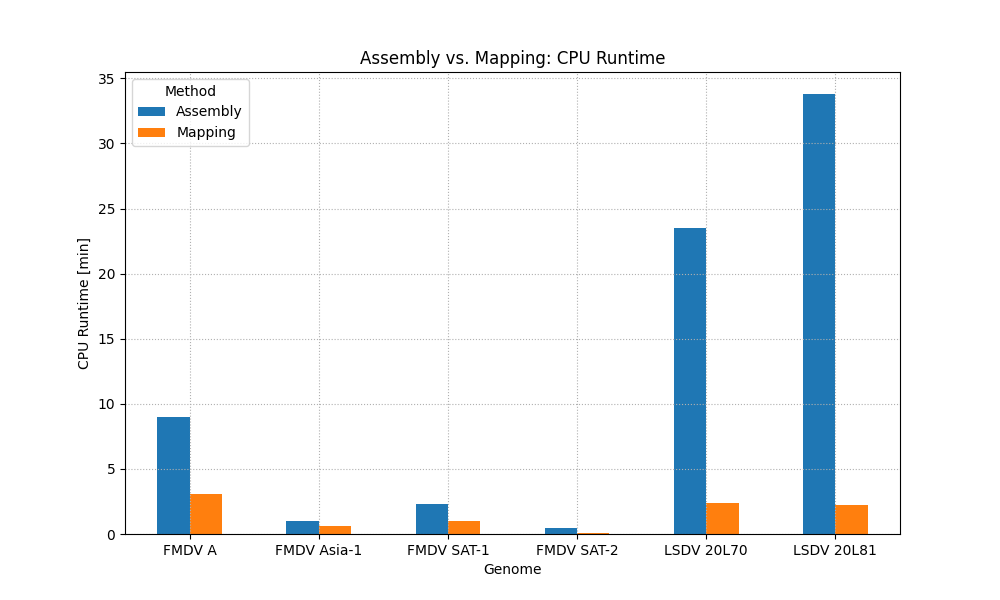
\includegraphics[width=1.0\textwidth]{media/4-profiling-cputime.png}
        \caption{Profiling of assembly vs. mapping, comparison of CPU runtimes for 4 FMDV and 2 LSDV samples.}
        \label{fig:4-profiling-cpu}
    \end{subfigure}
	\begin{subfigure}[b]{1.0\textwidth}
        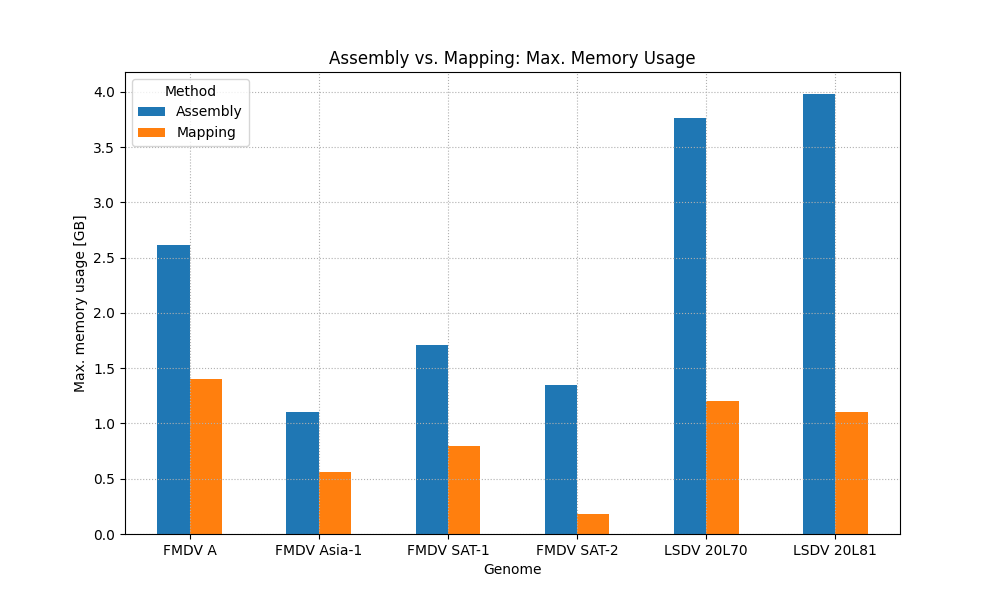
\includegraphics[width=1.0\textwidth]{media/4-profiling-maxmem.png}
        \caption{Profiling of assembly vs. mapping, comparison of maximal memory usage for 4 FMDV and 2 LSDV samples.}
        \label{fig:4-profiling-mem}
    \end{subfigure}
    \caption[Profiling of assembly vs. mapping.]{Profiling of assembly vs. mapping using viral genomes of different lengths.}
\end{figure}
\begin{figure}[ht!]\ContinuedFloat
    \centering
	\begin{subfigure}[b]{1.0\textwidth}
        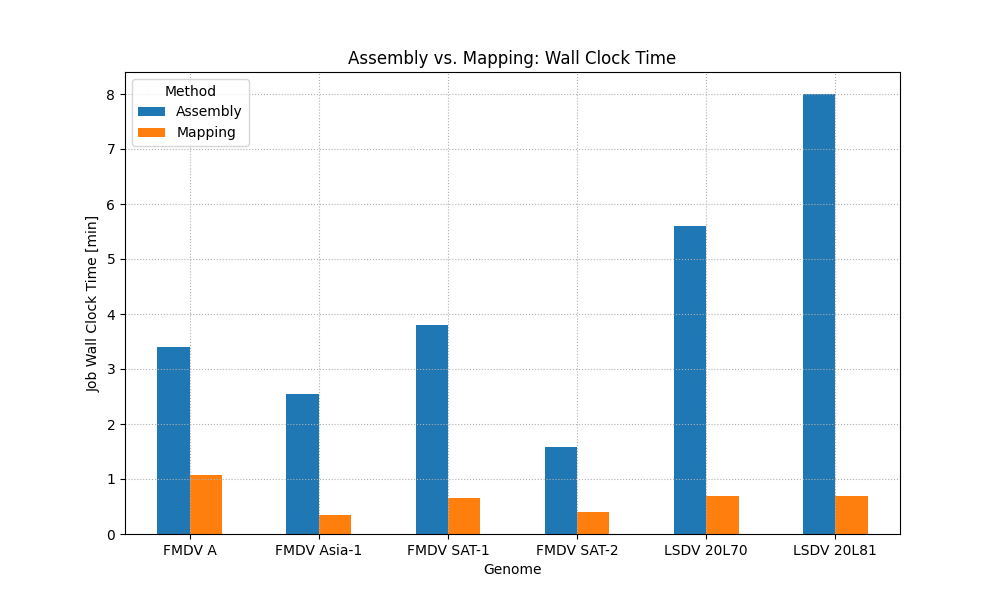
\includegraphics[width=1.0\textwidth]{media/4-profiling-wallclock.png}
        \caption{Profiling of assembly vs. mapping, comparison of job wall clock time which equals job execution time, for 4 FMDV and 2 LSDV samples.}
        \label{fig:4-profiling-wallclock}
    \end{subfigure}
	\begin{subfigure}[b]{1.0\textwidth}
        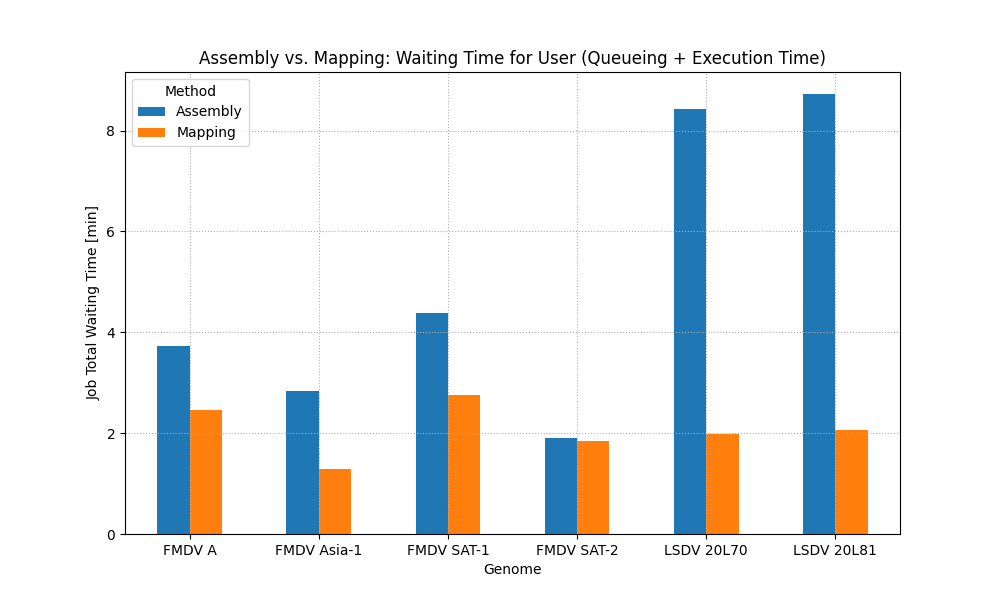
\includegraphics[width=1.0\textwidth]{media/4-profiling-total.png}
        \caption{Profiling of assembly vs. mapping, comparison of total waiting time for the job to finish for 4 FMDV and 2 LSDV samples.}
        \label{fig:4-profiling-total}
    \end{subfigure}
    \caption[Profiling of assembly vs. mapping (cont.).]{Profiling of assembly vs. mapping using viral genomes of different lengths (cont.).}
    \label{fig:apx-profiling}
\end{figure}
